\section{Rapport de fin d'itération}

Nous avons rencontré moins d'accrocs lors de cette phase que lors des deux premières. 
Aucun événement extérieur indépendant de notre volonté nous a bloqué, et nous 
avions toutes les cartes en main dès le début; cette itération fut donc une 
promenade de santé sur un long fleuve tranquille sans cascade ni haine ni 
violence dans la paix et l'entente de groupe les plus totales.


\subsection{Follow-up sur le rapport de fin d'itération précédente}
Dans le rapport de fin de l'itération précédente, nous mettions le doigt sur 
quelques problèmes qui nous ont été rappelés par la suite par les assistants.

	\subsubsection{Responsabilités du GeometryDAO (et d'autres classes)}
	Le \texttt{GeometryDAO}, classe centrale du projet, a grandi de manière 
	indésirable et presqu'incontrôlée jusqu'à l'itération 2. Son architecture 
	nous forçait à écrire beaucoup de méthodes spécifiques ou de tests de type 
	à beaucoup d'endroits du DAO. Nous avons réglé ce problème en créant une 
	Factory de DAO qui sera expliquée plus bas dans la section Architecture.\\

	Le WorldController a aussi été identifié comme étant une classe trop grande 
	et avec trop de responsabilités hétérogènes. Ce problème a été taclé grâce 
	à l'implémentation d'un pattern State, lui aussi décrit plus loin dans ce 
	rapport.

	\subsubsection{Documentation et tests}
	La documentation a été en grande partie complétée lors de cette itération. 
	Pour ce qui est des tests, nous utilisons de plus en plus le 
	\textit{test-driven development}; notamment dans l'écriture des Parsers pour 
	laquelle nous écrivions très vite des tests pour fixer leur comportement, 
	et aussi du \textit{regression testing} : nous écrivions un test à chaque 
	fois que nous nous heurtions à un comportement inattendu.

	\subsubsection{Meilleure répartition des packages}
	Il nous a été conseillé de répartir les classes par fonctionnalité plutôt
	que par "rôle" dans le pattern MVC. Cela a été fait.


\subsection{Suivi du planning}
Encore une fois, toute les fonctionnalités prévues ont été implémentées. Nous 
sommes également plutôt heureux d'avoir pu effectuer assez vite quelques 
refactorings importants. Bien que nous n'ayons pas peur de refactorer en plein 
développement, la période de début d'itération s'avère être un excellent moment 
pour remettre tout le projet au clair.


\subsection{Librairies introduites}

\paragraph{JDOM}
Nous avons décidé d'utiliser JDOM pour la manipulation de l'XML nécessaire dans
plusieurs formats. Cette libraire facilite grandement l'accès aux données, et 
semblait être reconnue à plusieurs endroits comme étant une référence en la matière.


\subsection{Architecture}
	
	\subsubsection{Rajouts dans le modèle}

		\paragraph{Rajout des parsers}
		Nous avons créé un \texttt{ImportEngine} qui va gérer les demandes 
		d'import de l'utilisateur et la création/gestion des différents parsers 
		à sa disposition. \\

		Chaque parser hérite de la classe \texttt{Parser} qui impose un comportement
		standard pour chacun d'entre eux. L'\texttt{ImportEngine} travaille dès
		lors très facilement avec des Parsers qui ont un comportement générique.
		Il faut donc très peu le modifier si on désire rajouter un Parser.\\

		L'architecture du système d'importation est visible à la figure \ref{fig:model:parsersarchi}.

		\begin{figure}
			\center
			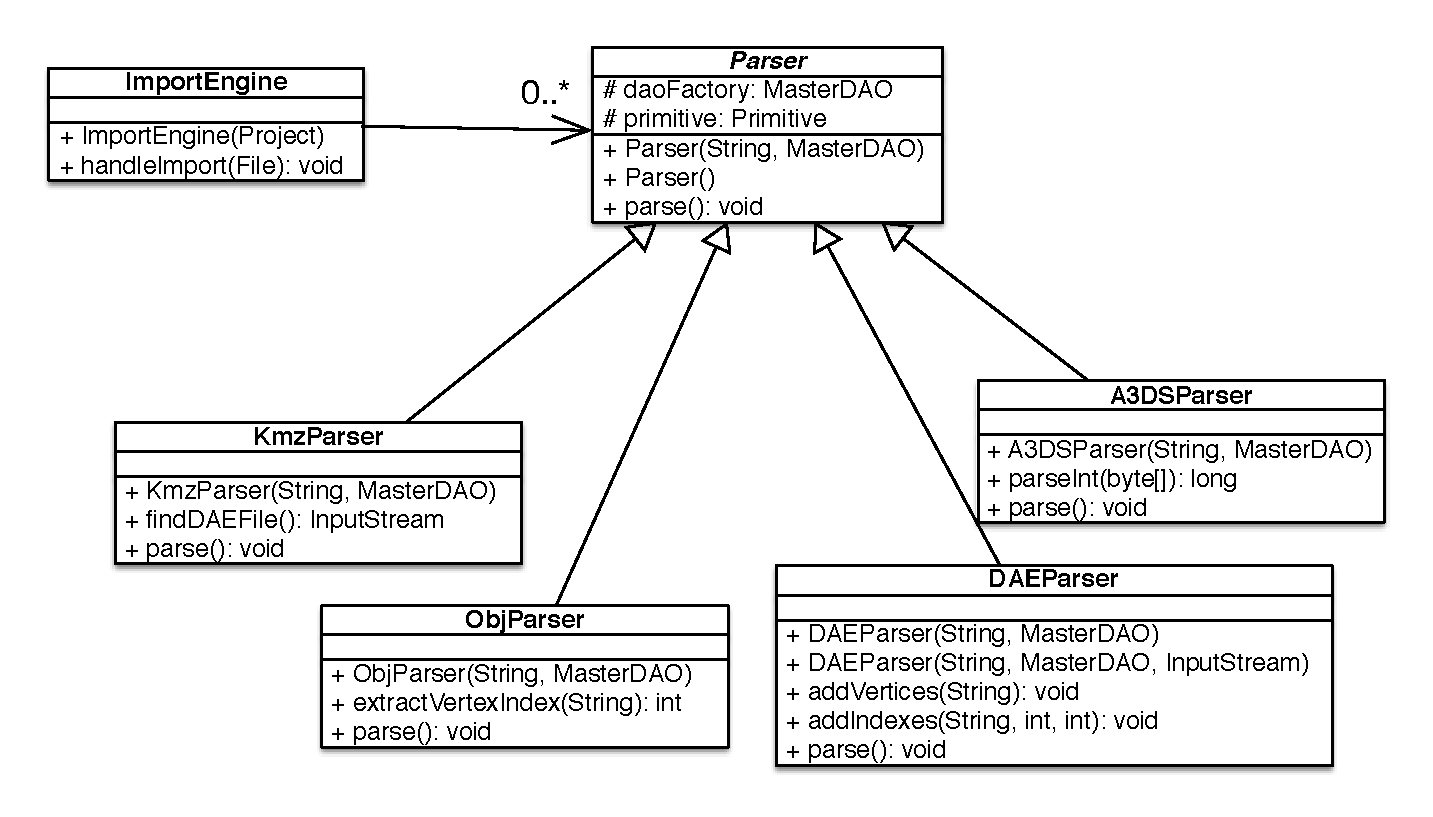
\includegraphics[width=\textwidth]{iteration3/fig/ParsersArchi.eps}
			\caption{\label{fig:model:parsersarchi} Architecture du système d'import}
		\end{figure}

		\paragraph{Rajout des exporters}
		À l'image de l'\texttt{ImportEngine}, nous avons aussi créé un 
		\texttt{ExportEngine} qui gère les demandes d'export de l'utilisateur et
		sa collection d'exporters.

		\paragraph{Primitives compatibles avec l'import/export}
		Le modèle supporte maintenant l'ajout de primitives non standard dans un
		Item qui sont désormais composées de Vertex et d'Indices (déterminant 
		les faces) afin de faciliter l'import/export d'objets qui ne sont pas des
		primitives de jMonkeyEngine.

	\subsubsection{Changements dans le modèle}

		\paragraph{Refactoring du GeometryDAO}
		La figure \ref{fig:model:olddaoclass} montre le diagramme de l'ancienne
		class GeometryDAO, et la figure \ref{fig:model:olddaointeraction} montre
		l'interaction que les vues et les contrôleurs avaient avec le DAO. On
		voit très clairement que l'ancien DAO dont la figure prend une page A4
		en hauteur avait trop de responsabilités et avait des méthodes beaucoup
		trop liées aux données qu'il manipulait (\texttt{getRoom()},...).\\

		Nous avons donc changé le GeometryDAO en MasterDAO qui est une Factory de 
		GeometricDAO génériques (figure \ref{fig:model:newdaoarchi}). Le MasterDAO 
		crée donc un GeometricDAO pour chaque type d'objet à insérer dans 
		la base de données. Les nouvelles interactions des vues et des contrôleurs 
		avec les DAO sont représentées en figure \ref{fig:model:newdaointeractions}.\\

		Chaque GeometricDAO retient son MasterDAO pour lui transférer les changements
		qu'il effectue, ce qui permet au MasterDAO d'ensuite les transférer à tous 
		ses Listener. On garde donc un seul lien vers le modèle
		dans les contrôleurs et les vues tout en découplant très fort son accès,
		et en rendant très facile le rajout de différents types d'objets.\\

		Prenons un exemple d'exécution en nous aidant de la figure \ref{fig:model:newdaointeractions}. Si un contrôleur veut changer un objet \texttt{Floor}, il demande au
		MasterDAO le \texttt{GeometricDao<Floor>}. Le contrôleur appelle la méthode
		\texttt{modify()} à laquelle il passe le \texttt{Floor} en question en paramètre.
		Le \texttt{GeometricDao<Floor>} prend en charge l'interaction avec la base
		de données, puis transfère le changement au MasterDAO; qui notifie tous
		les objets qui l'écoutent : toutes les vues sont donc mises au courant
		de la mise à jour.
		\begin{figure}
			\center
			\includegraphics[height=0.9\textheight]{iteration3/fig/OldGeometryDAO.png}
			\caption{\label{fig:model:olddaoclass} Vieux GeometryDAO}
		\end{figure}
		\begin{figure}
			\center
			\includegraphics[width=\textwidth]{iteration3/fig/OldDAOInteractions.png}
			\caption{\label{fig:model:olddaointeraction} Vieilles interactions avec le DAO}
		\end{figure}
		\begin{figure}
			\center
			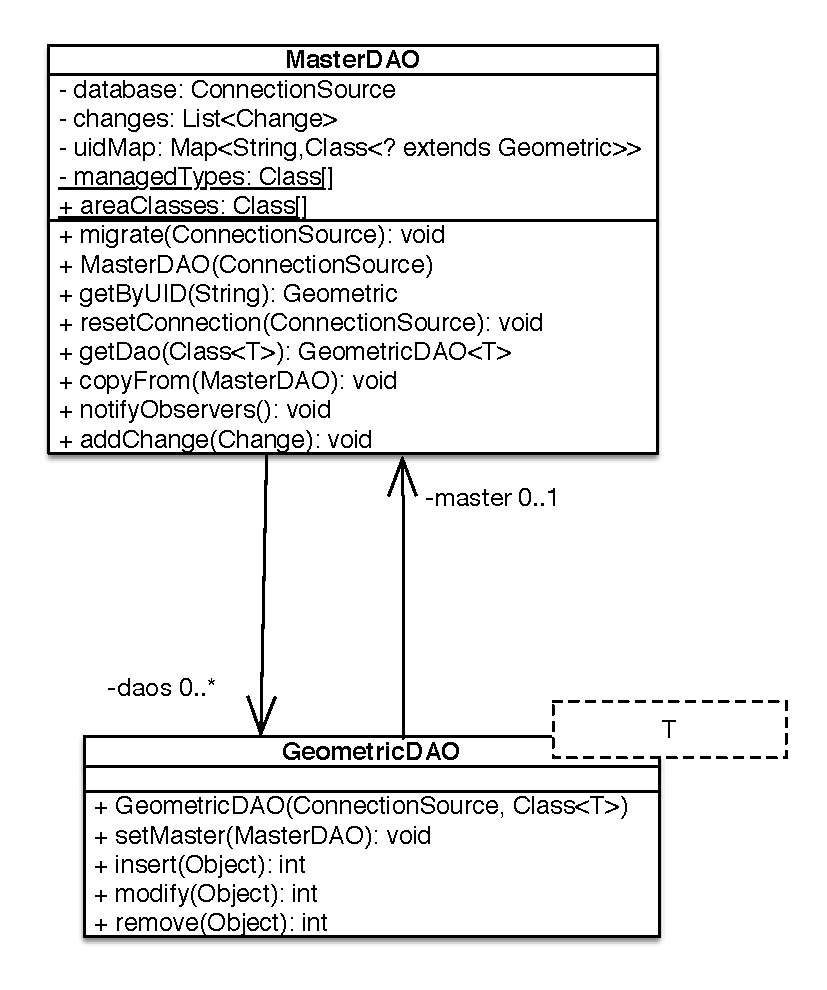
\includegraphics[width=0.5\textwidth]{iteration3/fig/NewDAOArchitecture.eps}
			\caption{\label{fig:model:newdaoarchi} Nouvelle architecture des DAO}
		\end{figure}
		\begin{figure}
			\center
			\includegraphics[width=\textwidth]{iteration3/fig/NewDAOInteractions.png}
			\caption{\label{fig:model:newdaointeractions} Nouvelles interactions avec les DAO}
		\end{figure}

	\subsubsection{Changements dans la GUI}

		\paragraph{Refactoring du WorldController}
		Au terme de la deuxième itération, le WorldController prenait en charge 
		la gestion du \textit{monde} (bâtiment, etc) et la gestion des objets.
		Ces 2 comportements n'étant pas liés logiquement et pouvant être séparés,
		tout en devant garder la même vue (le canevas jMonkey), nous avons séparé
		le WorldController en plusieurs classes grâce au pattern State.
		On peut voir un schéma minimaliste de cette nouvelle architecture en 
		figure \ref{fig:gui:newworldcontroller}.\\

		La WorldView a un contrôleur différent en fonction du mode d'édition
		dans lequel le programme se situe. 
		\begin{figure}
			\center
			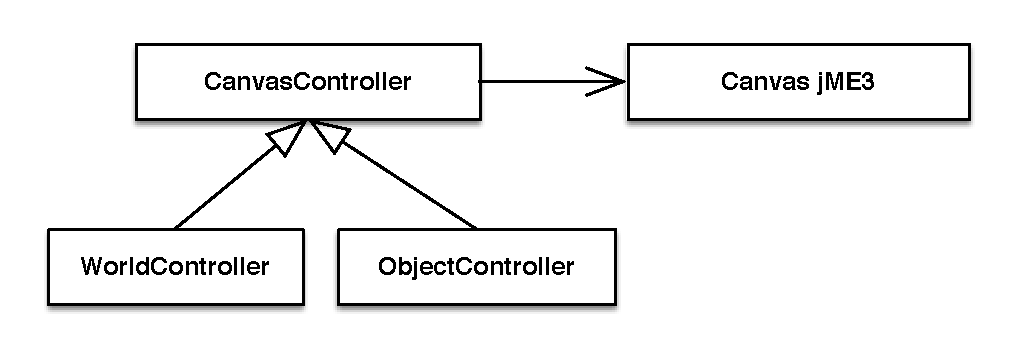
\includegraphics[width=0.5\textwidth]{iteration3/fig/WorldState.eps}
			\caption{\label{fig:gui:newworldcontroller} Architecture des contrôleurs de la WorldView}
		\end{figure}

	\subsubsection{Rajouts dans la GUI}

		\paragraph{Import/Export}
		Nous avons rajouté des menus d'import et d'export pour les objets.


\subsection{Bonnes pratiques - Outils}

	Outre les différentes techniques précisées dans les chapitres précédents, 
	nous avons développé plus intensément les pratiques suivantes.

	\paragraph{Pair programming}
	Nous avons utilisé cette technique de manière extensive. À peu près la moitié
	du projet a été écrite en pair programming. Généralement, tout ce qui était
	codé en solo n'était pas très fiable et buggait; ces parties ont été corrigées
	en pair programming.

	\paragraph{Regression testing}
	Le meilleur exemple de regression testing se trouve dans le développement des
	parsers. Ces morceaux de codes devant suivre des standards plutôt précis, nous
	nous sommes heurtés plusieurs fois à des problèmes spécifiques pour lesquels
	nous avons écrit des tests avant d'essayer de débugger le code.

\subsection{Conclusion - What's next}

	Cette itération s'est très bien déroulée. Nous ne pouvons plus nous plaindre
	de classe trop grande, dont les responsabilités mélangées se perdent les unes
	entre les autres. La fonctionnalité atteinte est encore très satisfaisante.

	\paragraph{Analyse de la classe Ordered}
	Les assistants nous ont glissé un mot quant à l'architecture autour de la
	classe Ordered et nous ont suggéré d'utiliser un design pattern. Nous analyserons
	ce problème lors de la prochaine itération.

	\paragraph{Optimisation des objets importés}
	Au vu de la taille des données manipulées avec les objets importés, certaines
	opérations prennent du temps et doivent être optimisées.
	
	\paragraph{Tests}
	Le code pourrait être mieux couvert par les tests, et malgré une allocation
	de plus en plus grande de temps pour l'écriture de tests, nous ne sommes pas
	encore satisfaits par la couverture.
	
	\paragraph{Finition}
	Certains bugs sans grosse conséquence sont présents dans le logiciel. Nous allons
	passer plus de temps lors de la prochaine itération pour en chasser un maximum.

